\section{Analysis of Trilateration}


As discussed in previous sections it is important to develop non-fingerprinting based solutions for indoor localization. Additionally, such solutions should preferably work with signal-strength information since they do not require additional hardware. Trilateration is a basic non-fingerprinting approach, which is robust and easy to implement but suffers from poor accuracy. However there is scope to adapt and improve trilateration. Towards this we have analyzed the performance and patterns in trilateration and identified the potential areas for improvement and this section goes into the details of this analysis. 

Firstly we discuss the target environment where we conducted our experiments to analyze the performance of trilateration. The target environment is a typical office space with several cubicles and pathways for walking which is analogous to normal indoor settings. Belkin N600 DB Wireless Dual Band N+ Routers were used to collect the dataset. To achieve the optimal coverage of the area, four routers are strategically placed such that the variance amongst them is maximum \cite{kaemarungsi2012analysis , CiscoLocation}. Additionally, the router's relative position from the ground also plays a pivotal role. The RSSI variance between routers influences the optimal positioning, and after analysis \cite{shanmugaapriyan2014pragmatic} , it was observed that for any point for precise localization  three routers at a maximum distance of 18 m away from each other were required. To eliminate any shadowing due to obstacles, the routers were placed up high ( 2.43m ) \cite{shanmugaapriyan2014pragmatic}, which also aids in maintaining a line of sight with minimum path loss at each point. Thus the routers were positioned as shown in \ref{fig:tenv}.

\begin{figure}[h]
\centering
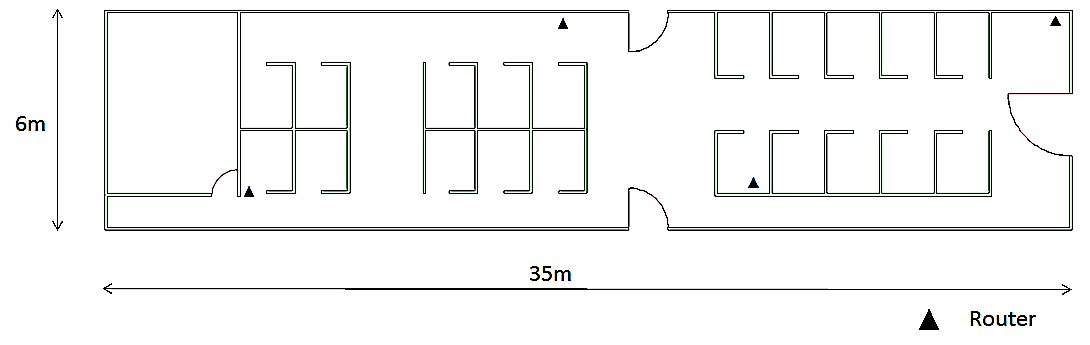
\includegraphics[width=80mm]{Tenv.png}
\caption{ Localization area 1 }
\label{fig:tenv}
\end{figure}

Several experiments were conducted in this environment, primarily for fingerprint data collection over several iterations and for localization experiments \cite{shanmugaapriyan2014pragmatic}. Additionally experiments were performed to understand the path-loss in different environments. Our analysis of the trilateration has been conducted over several of these experiment data sets.

In addition to this environment, to test out the veracity of our results we tested our algorithm in a much larger environment, which subsumes the office. The larger area contains corridor like walkways, several open spaces and a larger number of access points. We use commercially available off the shelf TP-LINK routers. The routers were strategically placed with the same positioning parameters considered in environment 1. The environment is illustrated in figure \ref{fig:tenv2}

\begin{figure}[h]
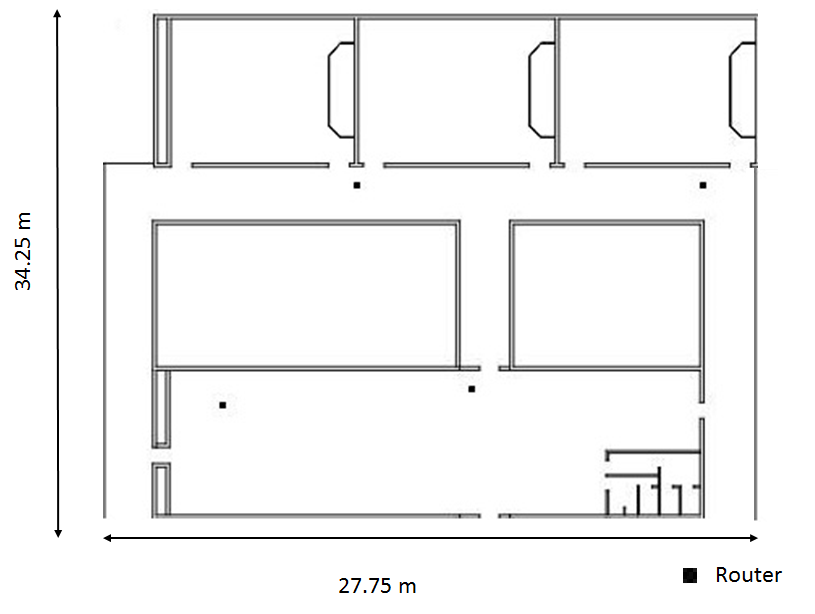
\includegraphics[width=25mm]{Tenv2.png}
\caption{ Localization area 2 }
\label{fig:tenv2}
\end{figure}

We first performed trilateration over several points in the fingerprint databases and calculated the overall accuracy \cite{shanmugaapriyan2014pragmatic}. On probing the results, we find that for the majority of the points the intersection region was inaccurate. Hence we used non linear least square regression to better find the probable region. In this environment, we noted an average accuracy of 7.76m with it being .64m in the best case and a terrible 21.49m in the worse case scenario. 
%, which is a method to approximate the modelling region to a linear one and refine it in succeeding iterations.
The accuracy definitely needs to be improved, therefore warranting further analysis. Upon further examination, it was discerned that the source of this discrepancy could be attributed to the error in distance estimation. Distance estimation is based on appropriate distance propagation models.

There are several propagation models that exist. Models such as Hata-Okamura, Log distance path loss, ITU etc. are dependent on the log-distance equation to model the signal path loss. These models are widely accepted due to being derivations of the free space path loss model, which originates from the inverse square law and the antenna gain. For our experiments, We consider the log distance path loss model as our RF propagation model \cite{sarkar2003survey, soorty2015finding}.

\begin{equation}
\Bigg[\frac{P_{L}(d)}{P_{L}(d_{0})}\Bigg]_{dB}  ~=~ -10n log\Bigg(\frac{d}{d_{0}}\Bigg) + X_{dB}
\label{pathlosseqn}
\end{equation}

where $PL(d0)$ is the total path loss measured in (dB) at a distance d0, $PL(d)$ is the total path loss measured in (dB) at the distance d1, n is path loss exponent (3 in our case) and 'X' is a zero mean Gaussian distributed random variable and since the shadowing effect in our experiments is inconspicuous and can be ignored, 'X' is equated to 0.

%While environmental factors cause the errors in trilateration, our goal is to identify the effects on trilateration and not analyze the cause i.e, we only look at the geometric patterns of the circles and their impact on the accuracy.  
%insert our graphs here - 
%add a para about the issues in path loss models . 

While the log distance path loss model takes shadowing into account, it still is founded upon empirically derived evidence and does not hold good in all environments. The path loss exponent is an important parameter and not choosing an appropriate value could considerably alter the end results \cite{srinivasa2009path}. Furthermore, the path loss exponent is prone to change with changes to the environment and is also affected by the obstacle density in room.
%In the case of an empty building, the value of the path loss exponent would shift towards the lower end of the spectrum. In such a case, the distance being estimated would be much lower than the one in in heavily dense environments, such as a file/stock room, where it would lean towards the higher end. In addition to this, the power of the signal drops when passing through walls. Thus in an office like environment where there are several partitions, the possibility of the signal attenuating is high and this may translate in a weaker signal and consequently a large distance being estimated even though the actual distance is low.
It can be observed that a lower path-loss exponent provides for better distance estimation in cluttered indoor spaces, but are prone to underestimations when the obstacles do not completely affect the line-of-sight. Higher path-loss exponents are better in near-line-of-sight environments, but prone to overestimation when obstacles like walls are there. 
Identification of these errors are difficult since it is based on environment and other factors. However it is possible to identify the type of issues causing these errors by observing the trilateration itself, i.e. by observing the geometric patterns of the circles used in trilateration. 
We shall explain our observation and how we characterize these observations from the trilateration patterns consequently.  It must be noted that these patterns can be identified only when the placement of routers follow standard guidelines and the path loss exponent is set after careful consideration. Errors due to bad placement and poor density of routers is beyond scope of this work, and therefore observations are based on the adherence to above requirements.

\subsection {Trilateration Patterns}
Our goal here is to identify the ramifications of these factors on trilateration and methods to alleviate the error, and not the factors themselves. For this, we look at the geometric patterns of the circles and their impact on the accuracy. Taking that into consideration, we look into the patterns in the overlapping circles. Consider the three circles $c1, c2$, and $c3$ in the trilateration with radius $r1, r2$ and $r3$ respectively. Our primary observations are as follows:
\begin{enumerate}
    \item Underestimation can be understood from the trilateration pattern based on the level of overlap. 
    \item  Overestimation can be discerned from some cases based on the level of overlap
    \item From the strength of RSSI and trilateration patterns we can determine if trilateration is the best approach for estimating a given point. 
    \item Due to underestimation, it is important to give higher probability to the outer parts of the disc in containing the original point than the center. However when overestimation is higher the probability should be given to the middle portion of the disc.
\end{enumerate}
The following paragraphs will explain these observations in detail. 

\textbf{Characterizing Underestimation:} As mentioned earlier underestimation occurs when estimated distance using the log-distance model is lower than the actual distance from the router, and is common in indoor scenarios. When observing the overlap of circles during trilateration, underestimation can be clearly determined when there is lack of overlap of some or all circles with other circles. When there is no overlap, a resizing of circles is required so that overlap occurs. 
\begin{definition}
If $c1 \cap c2= \pi 
\end{definition}
This distance re-estimation will be discussed in the next section. There are cases when overlap does not happen, it is because of underestimation in a few routers, but overestimation in others. However this case is difficult to characterize and deal with. We still treat these cases as underestimation, and account for this during circle resize. 
In the environments where we conducted our experiments we have found the out of around 80 points that were evaluated, 57\% of them had underestimation. Figure \ref{types_under} shows different types of underestimation as observed from the circles as discussed above.

\begin{table*}[h!]
\begin{tabular}{ | c | p{5cm} | p{5cm} | }
\hline
Two circle intersection & Relative intersection of two circles & No Intersection \\
\hline
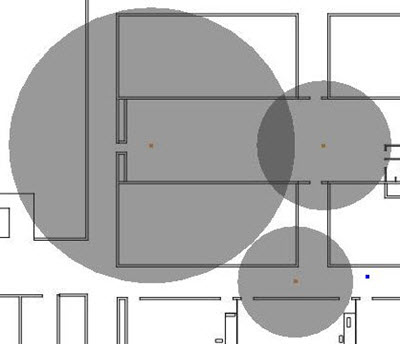
\includegraphics[width=0.15\textwidth, height=20mm]{Images/Two-Intersect.jpg}
& 
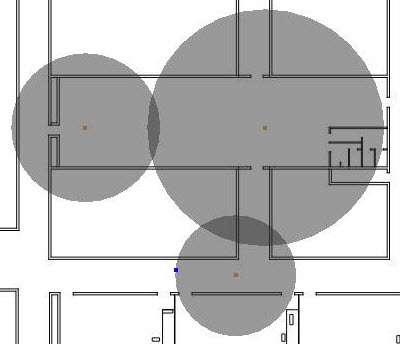
\includegraphics[width=0.15\textwidth, height=20mm]{Images/In-Between.jpg}
& 
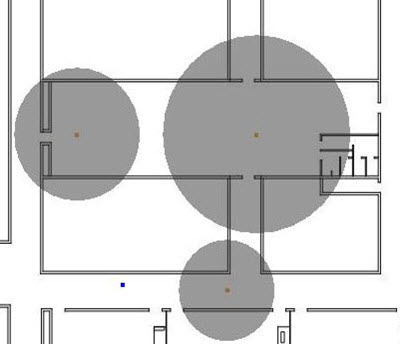
\includegraphics[width=0.15\textwidth, height=20mm]{Images/Non-Intersect.jpg}
\\ \hline
61\% of the cases & 1\% of the cases & 38\% of the cases
\\ \hline
\end{tabular}
\\
\caption{Underestimation Analysis}
\label{tbl:types_underest}
\end{table*}

\textbf{Determining Overestimation:} Overestimation usually results in a larger circle, therefore leading to a larger overlapping region. While there are several possible cases that indicate overestimation, many of these need not necessarily mean so. However in two types of overlap of the circles we can be confident of overestimation and these cases are 
a) a circle completely encloses another circle 
b) the percentage overlap between two circles is greater than a predefined threshold, and the third circle is not disconnected from the others. 
In both these cases the overestimation occurs mostly in the largest circle(s) and their radii have to be reduced proportionately. In other cases usually trilateration should estimate the position reasonable well.

In our environment 1 we have found very little cases of overestimation. However more cases are seen in the larger environment and we find around 51\% of them are overestimated.

\textbf{Trilaterability of a point:} When the original point is near a router, it's signal strength is usually high. However, since the circle is very small, and the distance is far from the other routers, the circle overlap is skewed and the trilateration area is rarely close to the point. Additionally issues in error estimation as mentioned above complicates the overlap, leading to major localization errors. In such cases we observe that one circle is relatively much smaller compared to the other circles. When this circle is an over-estimation, the point is inside the smallest circle, and if it is an under-estimation, the point is generally outside of all three circles, and resizing may not help much. In some cases the points are away from the influence of other two routers. These cases can be see in Figure\ref{collageofpoints}. Classifying such points are non-trilaterable can help choose other techniques to estimate positions. In our environment we have found that around 43\% of the points fall in this category and therefore must be identified and addressed differently. 

It must be noted that there are cases where trilateration can work for such cases, however not doing trilateration does not affect accuracy drastically as we will see in the next section. 

\begin{figure}[ht!]
\centering
\includegraphics[width=80mm]{Images/Router Points.jpg}
\caption{ Trilaterability of a point}
\label{collageofpoints}
\end{figure}

% need examples , and figures for where trilateration fails here...

\textbf{Anomalous Centroid Position:} When trilateration occurs, the estimated point is the centroid of the overlapping area of the three circles. If the overlap is high due to errors discussed above, it is possible that the estimated point is located more towards the center of any circle. However when underestimation or correct estimation occurs, the point lies in the area around the border. If an overestimation occurs, the point may lie very close to the middle band of the circle. It is rare that the final point lies in the center of any disk and usually this occurs in the case when the point is very close to a router as discussed above. The figure\ref{collageofpoints1} shows these cases. During trilateration if this is accounted for, accuracy in estimation can be improved. 


\begin{figure}[ht!]
\centering
\includegraphics[width=80mm]{Images/Anomalous Centroid.jpg}
\caption{  }
\label{collageofpoints1}
\end{figure}

In our paper we use these findings to propose a Weighted Adaptive Location Estimation (WALE) algorithm that combines a probabilistic weighting approach with a dynamic circle resizing approach. The approach is customized based on whether a point is trilaterable or not. The next section will explain our algorithm in detail. 
